\section{Splay Trees}
\subsection{Definition}
\begin{itemize}
    \item binärer Suchbaum
    \item nach Zugriff auf Knoten $\rightarrow$ dieser zur Root
    \item Inorder-Traversierung retourniert die Keys in geordneter Folge
\end{itemize}

\subsection{Laufzeit}
Splaying-Cost: O(h)
\begin{itemize}
    \item Durschnittlich: O(log n)
    \item Worst Case: O(n)
\end{itemize}

\subsection{Splaying}
\begin{itemize}
    \item neue operation: splay
    \item Rotationen nach jeder Operation (sogar bei der Suche)
    \item Bewegen eines Knoten zur Root unter Benutzung von Rotationen
\end{itemize}

\begin{itemize}
    \item x ist das linke Kind von seinem Eltern-Knoten, welcher selber ein rechtes Kind ist von seinem Eltern-Knoten
    \item y ist x’s Eltern-Knoten
    \item z ist y’s Eltern-Knoten
\end{itemize}

\vspace{-8pt}
\begin{center}
    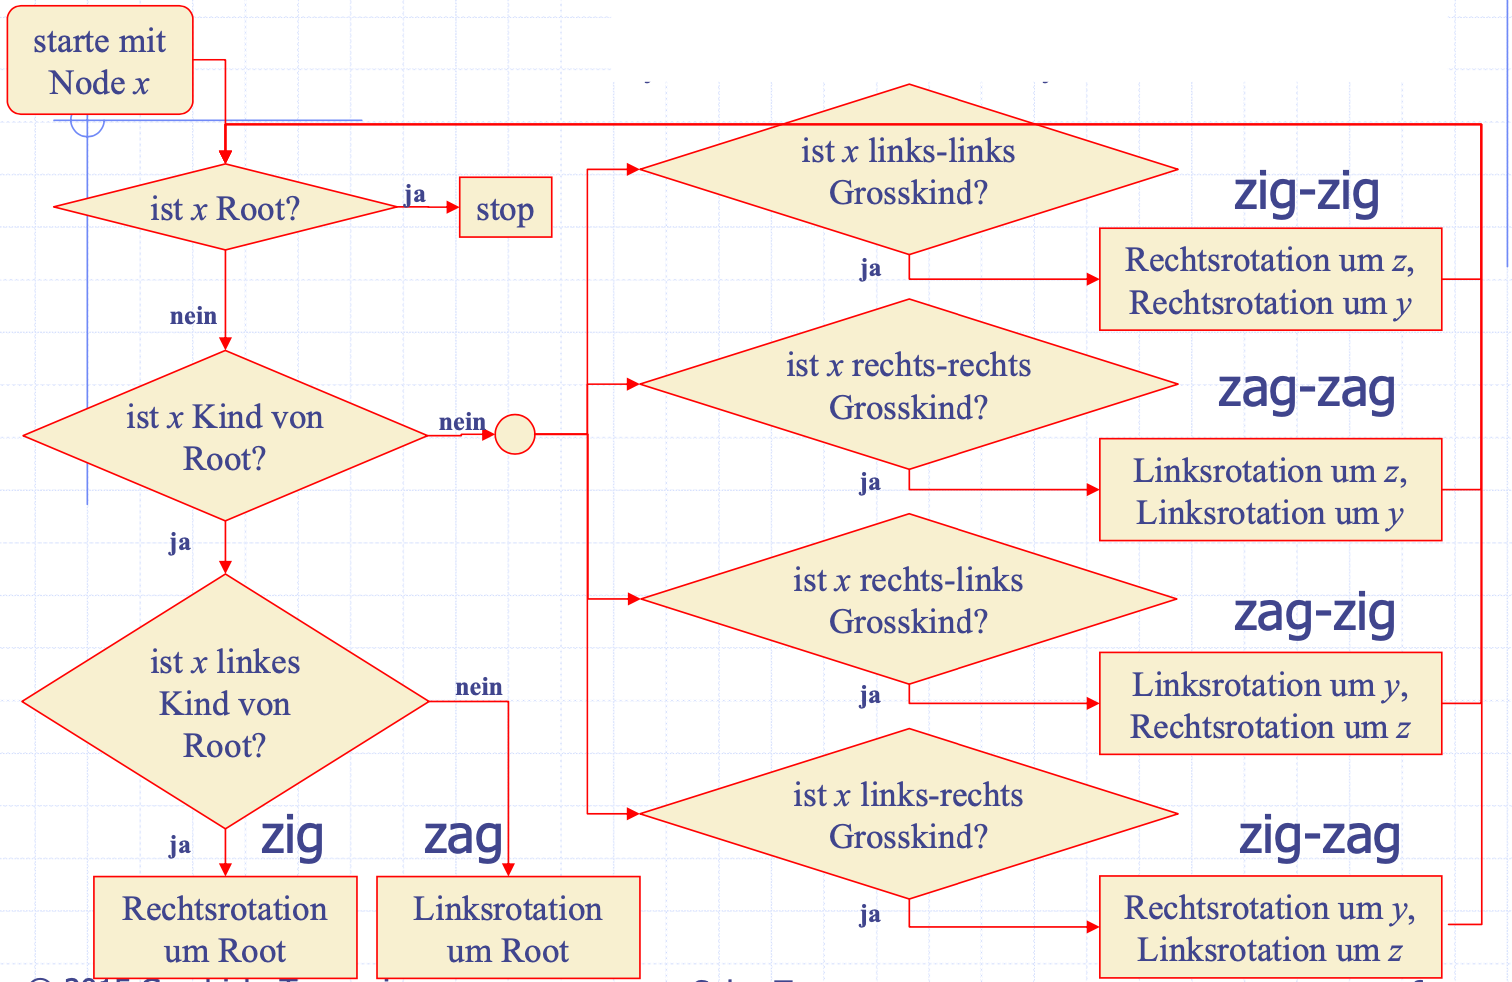
\includegraphics[scale=.2]{graphic/03 SplayTrees/splay.png}
    \includegraphics[scale=.2]{graphic/03 SplayTrees/splay fälle.png}
\end{center}
\vspace{-8pt}

\subsection{Suchen}
Suche geht den Baum abwärts bis zu einem gesuchten Entry oder einem externer Knoten

\subsection{Löschen}
\begin{center}
    \includegraphics[scale=.2]{graphic/03 SplayTrees/löschen}
\end{center}
\vspace{-8pt}

\subsection{Wer wird gesplayed?}
\begin{center}
    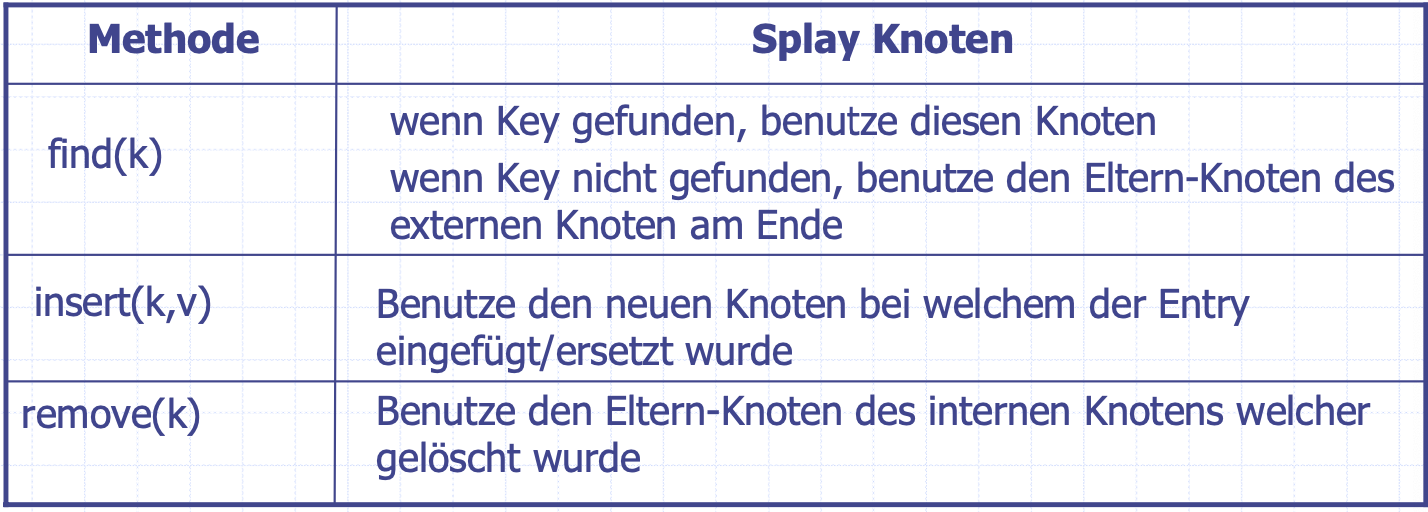
\includegraphics[scale=.25]{graphic/03 SplayTrees/who.png}
\end{center}

